\documentclass[a4paper]{article}
\addtolength{\hoffset}{-2.25cm}
\addtolength{\textwidth}{4.5cm}
\addtolength{\voffset}{-3.25cm}
\addtolength{\textheight}{5cm}
\setlength{\parskip}{0pt}
\setlength{\parindent}{0in}

\usepackage[square,sort,comma,numbers]{natbib}
\usepackage{blindtext} % Package to generate dummy text
\usepackage{charter} % Use the Charter font
\usepackage[utf8]{inputenc} % Use UTF-8 encoding
\usepackage{microtype} % Slightly tweak font spacing for aesthetics
\usepackage{amsthm, amsmath, amssymb} % Mathematical typesetting
\usepackage{float} % Improved interface for floating objects
\usepackage{hyperref} % For hyperlinks in the PDF
\usepackage{graphicx, multicol} % Enhanced support for graphics
\usepackage{xcolor} % Driver-independent color extensions
\usepackage{pseudocode} % Environment for specifying algorithms in a natural way
\usepackage[mmddyy]{datetime} % Uses YEAR-MONTH-DAY format for dates

\usepackage{fancyhdr} % Headers and footers
\pagestyle{fancy} % All pages have headers and footers
\fancyhead{}\renewcommand{\headrulewidth}{0pt} % Blank out the default header
\fancyfoot[L]{} % Custom footer text
\fancyfoot[C]{} % Custom footer text
\fancyfoot[R]{\thepage} % Custom footer text
\newcommand{\note}[1]{\marginpar{\scriptsize \textcolor{red}{#1}}} % Enables comments in red on margin

\DeclareMathOperator*{\argmin}{arg\,min}

%----------------------------------------------------------------------------------------


%-------------------------------
%	TITLE VARIABLES (identify your work!)
%-------------------------------

\newcommand{\yourname}{Nathan Ugwonali} % replace YOURNAME with your name
\newcommand{\youremail}{nathan.ugwonali@ens-paris-saclay.fr} % replace YOUREMAIL with your email
\newcommand{\assignmentnumber}{6} % replace X with the lab session number

\begin{document}

%-------------------------------
%	TITLE SECTION (do not modify unless you really need to)
%-------------------------------
\fancyhead[C]{}
\hrule \medskip
\begin{minipage}{0.295\textwidth} 
\raggedright
\footnotesize
\yourname \hfill\\
\youremail
\end{minipage}
\begin{minipage}{0.4\textwidth} 
\centering 
\large 
Lab session \# \assignmentnumber\\ 
\normalsize 
ALTEGRAD 2023\\ 
\end{minipage}
\begin{minipage}{0.295\textwidth} 
\raggedleft
\today\hfill\\
\end{minipage}
\medskip\hrule 
\bigskip



%-------------------------------
%	ASSIGNMENT CONTENT (add your responses)
%-------------------------------

\section{Question 1}

\paragraph{Setting.} Let $E \in \mathbb{R}^{11 \times h_1}$ be the embedding table (row $E_d$ for digit $d \in \{0, \dots, 10\}$, where $0$ is the padding symbol), $W_1 \in \mathbb{R}^{h_2 \times h_1}$, $b_1 \in \mathbb{R}^{h_2}$ the parameters of the first fully-connected layer, and $w_2 \in \mathbb{R}^{h_2}$, $b_2 \in \mathbb{R}$ those of the output layer. The model computes
\begin{equation}
    \phi(d) = \tanh(W_1 E_d + b_1), \qquad f(X) = w_2^\top \sum_{x \in X} \phi(x) + b_2 ,
\end{equation}
and we want $f(X) = \sum_{x \in X} x$ for every multiset $X$, padded or not.

\paragraph{Optimal parameters.} Since $\rho$ is a single affine layer, the sum must already be encoded linearly in $\sum_x \phi(x)$, so $\phi$ must be \emph{linear} in the digit: $\phi(d) \propto d$. It cannot be the identity, because $\tanh$ takes values in $(-1, 1)$, so we scale the digits by a constant $c > 10$ (e.g.\ $c = 11$) so that $d/c \in [0, 1)$ for every $d \in \{0, \dots, 10\}$. Using a single coordinate $k$ of the hidden layer, the expected solution is
\begin{align}
    &\text{fc1:} && b_{1,k} = 0, \quad (W_1)_{k,:}\, E_d = \tanh^{-1}\!\Big(\frac{d}{c}\Big) \ \ \forall d \in \{0, \dots, 10\}
        \quad\Longrightarrow\quad \phi(d)_k = \frac{d}{c}, \label{eq:phi}\\
    &\text{fc2:} && w_2 = c\, e_k \ \ (\text{weight } c \text{ on coordinate } k, \ 0 \text{ elsewhere}), \qquad b_2 = 0 .
\end{align}
The embedding is a free lookup table, so it can absorb the nonlinearity: it stores $\tanh^{-1}(d/c)$ along the direction $(W_1)_{k,:}$, which the $\tanh$ maps back to $d/c$. In particular, $d = 0$ gives $E_0 = 0$ (or any vector orthogonal to $(W_1)_{k,:}$), hence $\phi(0)_k = 0$. Then
\begin{equation}
    f(X) = c \sum_{x \in X} \phi(x)_k + 0 = c \sum_{x \in X} \frac{x}{c} = \sum_{x \in X} x .
\end{equation}
The other coordinates of $\phi$ are arbitrary, since $w_2$ gives them weight $0$.

\paragraph{Why these constraints.}
\begin{itemize}
    \item \textbf{Strict scaling ($c > 10$).} $\tanh^{-1}$ is only defined on $(-1, 1)$: with $c = 10$, the digit $10$ would require $\tanh^{-1}(1) = +\infty$.
    \item \textbf{No offset in $\phi$.} An affine encoding $\phi(d)_k = \alpha d + \beta$ with $\beta \neq 0$ (e.g.\ mapping $\{1, \dots, 10\}$ onto $[-1, 1]$) gives $\sum_{x \in X} \phi(x)_k = \alpha S + \beta\, |X|$ with $S = \sum_{x \in X} x$, which depends on the cardinality $|X|$; a fixed $\rho$ cannot remove this term since it does not know $|X|$.
    \item \textbf{$\phi(0) = 0$ on coordinate $k$.} Padding zeros must not contribute to the sum.
    \item \textbf{$b_2 = 0$.} The bias of $\rho$ is added once, after the sum; any nonzero value shifts every prediction.
\end{itemize}

\section{Question 2}

Both sets have the same sum, $[0.4, -0.2]^\top$, so no linear $\phi(x) = Wx + b$ can separate them: $\sum_{x} \phi(x) = W \sum_x x + 2b$ is identical for $X_1$ and $X_2$. A nonlinearity in $\phi$ is required. Take $\phi(x) = \mathrm{ReLU}(Wx + b)$ with $W = I$, $b = 0$, and $\rho$ the identity ($W_\rho = I$, $b_\rho = 0$):
\begin{align}
    X_1 &: \ \phi([1.2, -0.7]^\top) + \phi([-0.8, 0.5]^\top) = [1.2, 0]^\top + [0, 0.5]^\top = [1.2, 0.5]^\top, \\
    X_2 &: \ \phi([0.2, -0.3]^\top) + \phi([0.2, 0.1]^\top) = [0.2, 0]^\top + [0.2, 0.1]^\top = [0.4, 0.1]^\top .
\end{align}
The two embeddings differ, so this DeepSets model maps $X_1$ and $X_2$ to different vectors.


\section{Question 3}

Yes. Node orderings are arbitrary, so any function of a multiset of nodes inside a GNN must be permutation invariant, which is exactly what DeepSets models. It appears at two levels:
\begin{itemize}
    \item \textbf{Neighbourhood aggregation.} Each message passing layer updates $h_v$ from the multiset $\{h_u : u \in \mathcal{N}(v)\}$, which preserves the graph structure. GIN makes the analogy explicit: $h_v \leftarrow \mathrm{MLP}\big((1+\epsilon) h_v + \sum_{u \in \mathcal{N}(v)} h_u\big)$, i.e.\ a sum over the neighbours followed by $\rho = \mathrm{MLP}$.
    \item \textbf{Readout.} For graph classification, the node embeddings, which already encode the structure, must be pooled into a single graph vector independently of the node ordering. A DeepSets module $\rho\big(\sum_{v \in V} \phi(h_v)\big)$ is a natural readout, and the sum readout followed by an MLP is a special case.
\end{itemize}


\section{Question 4}

Relabelling the nodes with a permutation matrix $P$ maps $(A, X)$ to $(PAP^\top, PX)$.

\paragraph{Encoder.} The message passing layers are permutation \emph{equivariant}: the node embeddings become $PH$. The final sum over the nodes then receives the same multiset of vectors in a different order, so the graph-level output (hence $\mu$, $\log\sigma^2$ and $z$) is \emph{invariant}.

\paragraph{Reconstruction loss.} Each decoder logit is tied to a fixed position $(i, j)$, $i < j$, and the BCE compares it entry-wise with $A_{ij}$. Under a relabelling, the prediction is unchanged (since $z$ is invariant) but the target becomes $PAP^\top$, so the same graph yields different losses: the model is penalised for producing the right graph in another node ordering. An invariant loss would require a minimum over the $n!$ orderings (graph matching), which is intractable; a fixed node ordering is used instead.

\paragraph{BFS ordering.} No. A canonical ordering must give every isomorphic copy of a graph the same adjacency matrix, which is as hard as graph isomorphism. Degree-guided BFS breaks ties between nodes of equal degree by node index (keys $(\deg v, -v)$ and $(-\deg u, u)$), i.e.\ by the arbitrary input labelling. Two isomorphic copies with different labels can thus get different orderings, especially in near-regular graphs such as Watts--Strogatz with low rewiring, where many degrees tie. It only reduces the ordering ambiguity heuristically.


\section{Question 5}

Let $P$ be the decoded edge probability matrix. Thresholding sets $\hat{A}_{ij} = \mathbb{1}[P_{ij} > 0.5]$ (deterministic), whereas sampling draws $\hat{A}_{ij} \sim \mathrm{Bernoulli}(P_{ij})$ independently for each pair $i < j$ (stochastic).

\paragraph{Diversity.} Thresholding maps a given $P$ to a single graph, its most likely one; diversity can only come from varying $z$. Bernoulli sampling can produce any of the $2^{n(n-1)/2} = 2^{276}$ adjacency matrices when $0 < P_{ij} < 1$, concentrated around the expected graph, which is what a generative model of $p(G \mid c)$ should do.

\paragraph{Density.} Under sampling, $\mathbb{E}[\hat{A}_{ij}] = P_{ij}$, so the expected number of edges is $\sum_{i<j} P_{ij}$ and a calibrated $P$ preserves the requested density. Thresholding instead yields the fraction of entries above $0.5$, which pushes graphs to the extremes: for our sparse graphs ($\rho \in [0.12, 0.30]$), a calibrated $P$ with $P_{ij} \approx 0.2$ gives an almost empty graph, while entries slightly above $0.5$ all become edges. Thresholding thus systematically misses the density condition. On the other hand, independent Bernoulli edges ignore correlations between edges, so triangles (three edges appearing jointly) may be under-represented, which affects $t(G)$.


\section{Task 10: upper-triangular decoder}

The decoder outputs one logit per unordered pair $i < j$, i.e.\ $n(n-1)/2 = 276$ values, which are written at positions $(i, j)$ of a zero matrix and mirrored to $(j, i)$. No logit is ever assigned to a diagonal entry, so $P_{ii} = 0$ by construction and no self-loop can be sampled. Each undirected edge is predicted by a single logit, so $P$ is symmetric by construction: the model cannot give two inconsistent probabilities to $(i, j)$ and $(j, i)$, and the reconstruction loss does not count each edge twice.


\section{Task 12: conditional generation results}

One graph is sampled (Bernoulli edges) for each of $100$ held-out test requests, with $\beta = 0.005$. Mean absolute errors, averaged over 3 seeds (13, 14, 15), with the density-matched Erd\H{o}s--R\'enyi baseline ($p = \rho$):

\begin{center}
\begin{tabular}{l|c|c}
     & MAE density & MAE triangles/node \\
    \hline
    cVAE, $\lambda = 0$    & $0.0199$ & $0.352$ \\
    cVAE, $\lambda = 0.02$ & $0.0204$ & $\mathbf{0.311}$ \\
    ER baseline            & $0.0202$ & $0.401$ \\
\end{tabular}
\end{center}

Requested vs.\ achieved $(\rho, t)$ for the first five requests (seed 13, $\lambda = 0.02$):
\begin{center}
\begin{tabular}{c|c|c}
    Requested & cVAE & ER baseline \\
    \hline
    $(0.145, 0.250)$ & $(0.185, 0.625)$ & $(0.156, 0.417)$ \\
    $(0.174, 0.708)$ & $(0.170, 0.125)$ & $(0.127, 0.167)$ \\
    $(0.261, 1.167)$ & $(0.225, 0.792)$ & $(0.290, 2.292)$ \\
    $(0.217, 0.792)$ & $(0.217, 0.917)$ & $(0.188, 0.500)$ \\
    $(0.261, 1.375)$ & $(0.221, 1.167)$ & $(0.293, 2.208)$ \\
\end{tabular}
\end{center}

\begin{center}
    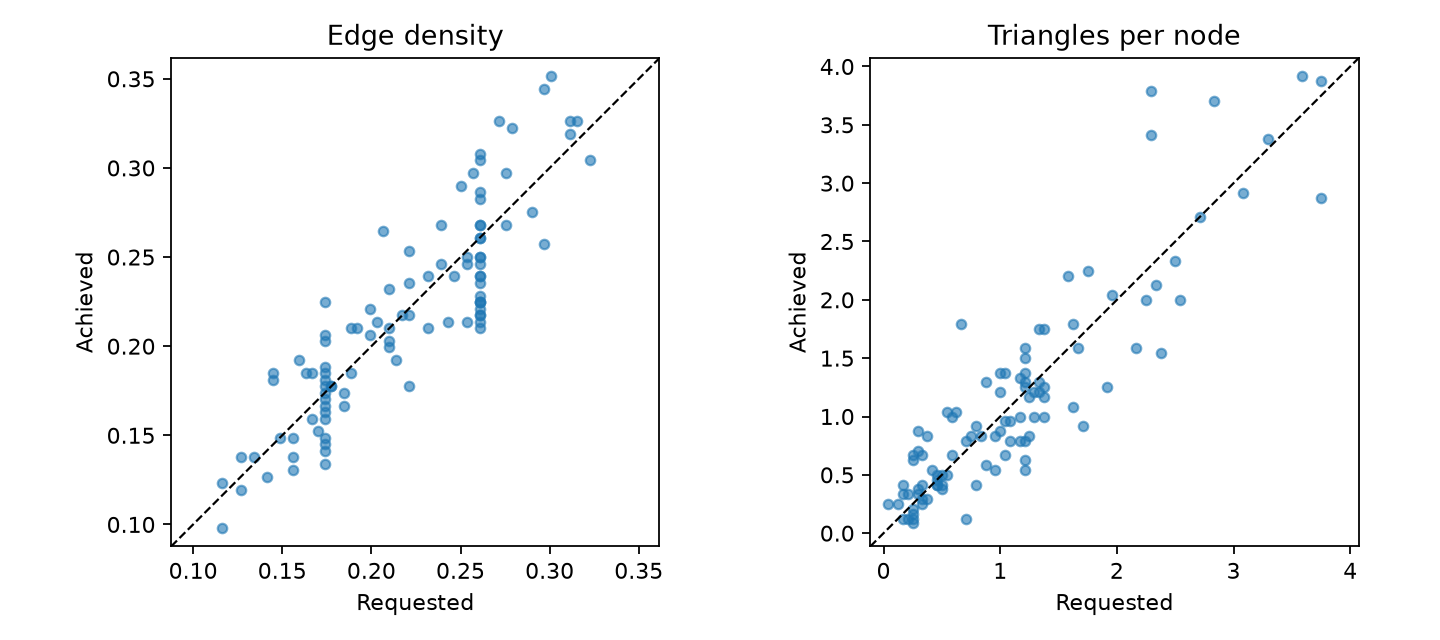
\includegraphics[width=0.8\linewidth]{figures/cvae_lambda002_requested_vs_achieved.png}
\end{center}

Both the cVAE and the baseline match the density equally well (MAE $\approx 0.02$): density is the easy property, and ER with $p = \rho$ matches it in expectation by design. The difference is in the triangles: ER has no separate control over $t(G)$, its expected number of triangles per node is fixed by $p$ alone, $\mathbb{E}[t] = \frac{(n-1)(n-2)}{6} p^3$ (e.g.\ $\approx 1.5$ for $\rho = 0.261$, whatever the requested $t$), whereas the cVAE reduces the triangle MAE by about $12\%$ ($\lambda = 0$) and $22\%$ ($\lambda = 0.02$). The property loss consistently lowers the triangle error (on all three seeds) at no cost in density. The errors remain substantial, as expected from Q5: a single Bernoulli sample with independent edges only matches the requested properties in expectation.


%------------------------------------------------

\end{document}
